%This is the first chapter of the dissertation

%The following command starts your chapter. If you want different titles used in your ToC and at the top of the page throughout the chapter, you can specify those values here. Since Columbia doesn't want extra information in the headers and footers, the "Top of Page Title" value won't actually appear.

\chapter[][Recursive Jigsaw Reconstruction]{Recursive Jigsaw Reconstruction}

\textit{Recursive Jigsaw Reconstruction} (RJR) \cite{Jackson:2016mfb,ATLAS-CONF-2016-078} is a novel algorithm used for the analysis presented in this thesis.
RJR is the conceptual successor to the razor technique \cite{Rogan:2010kb,Buckley:2013kua}, which has been used successfully in many new physics searches \cite{SUSY-2014-05,SUSY-2014-06,CMS-SUS-13-004,CMS-SUS-12-005,CMS-SUS-11-024,SUSY-2011-22}.
In this chapter, we will first present the razor technique, and describe the razor variables.
We will then present the RJR algorithm.
After the description of the algorithm, we will describe the precise RJR variables used by this thesis and attempt to provide some physical intuition of what they describe.

\section{Razor variables}

\subsection{Motivation}
In this thesis, we consider SUSY models where gluinos and squarks are pair-produced.
Pair-production is a consequence of the $R$-parity imposed in many SUSY models.
$R-$parity violation is highly constrained by limits on proton decay\todo{CitE}, and is often assumed in SUSY model building.
The Feynmann diagrams considered are shown in Fig.\ref{fig:feynmann_signal}.\todo{Check on W production thing, LO naming}.
\begin{figure}
\caption{Leading order Feynman diagrams for the SUSY signals considered in this thesis} \label{fig:feynmann_signal}
\subfloat[Disquark production]   {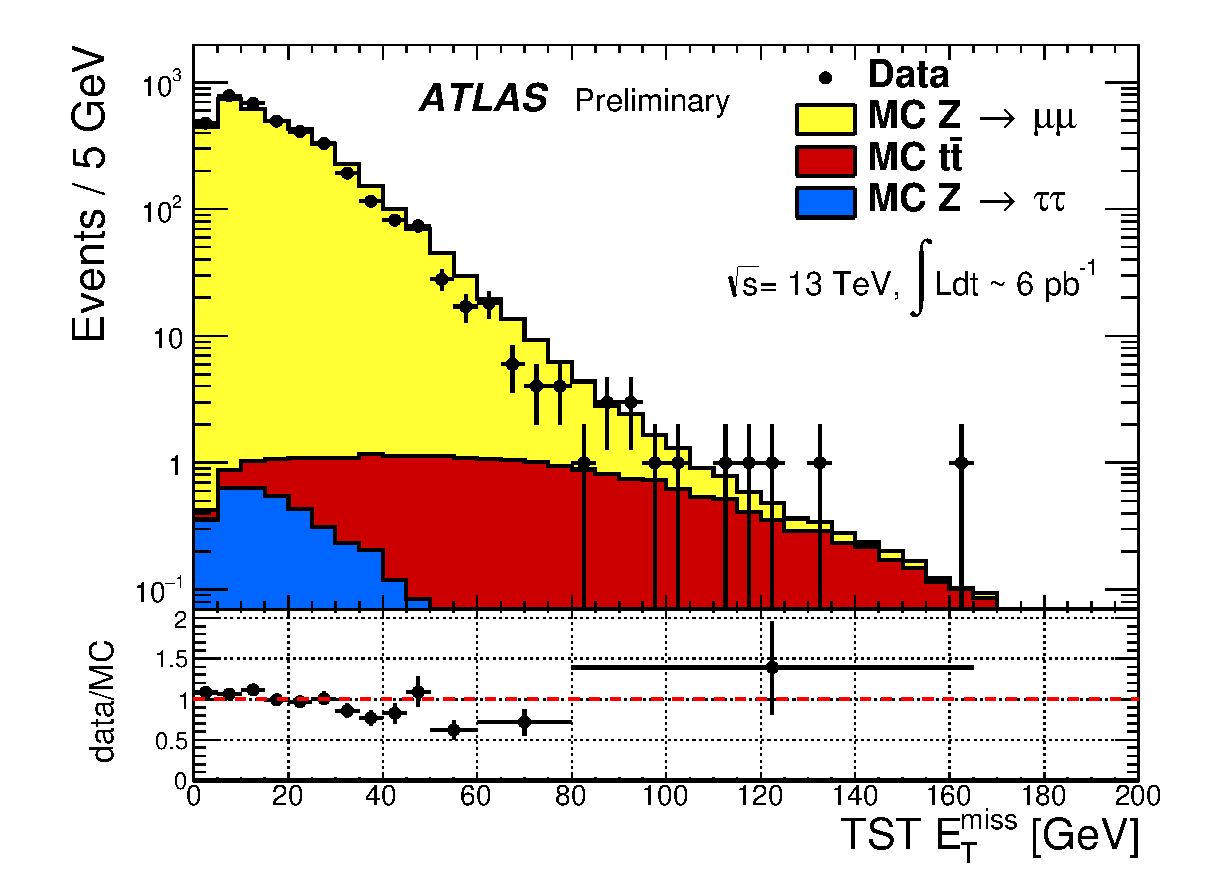
\includegraphics[width=.9\linewidth]{ATLAS-CONF-2016-078/fig_01a}} \\
\subfloat[Digluino production]   {\includegraphics[width=.9\linewidth]{ATLAS-CONF-2016-078/fig_01b}} \\
\subfloat[Digluino production with associated W bosons.]   {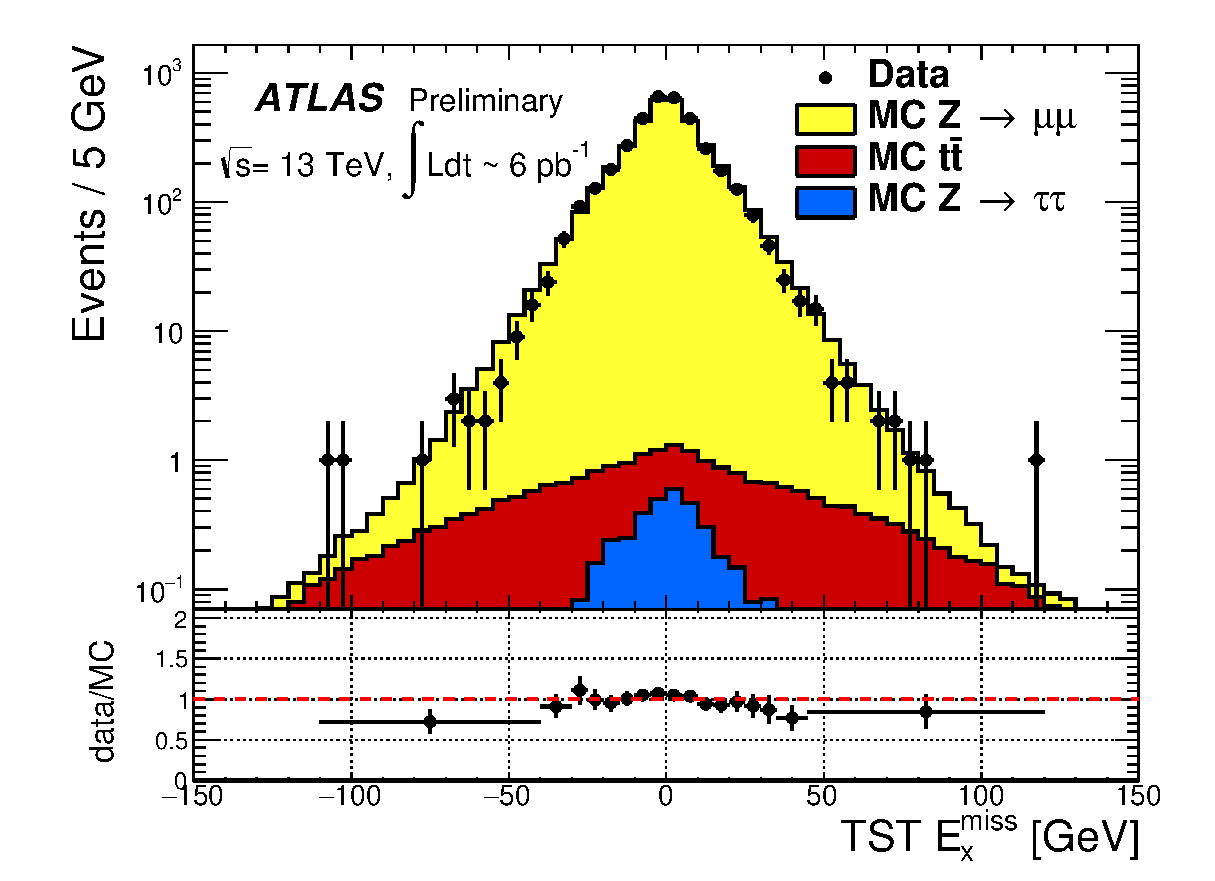
\includegraphics[width=.9\linewidth]{ATLAS-CONF-2016-078/fig_01c}}
\end{figure}

As discussed previously, the consequences of this $\mathbb{Z}_2$ symmetry are drastic.
To understand the utility of the razor variables, the stability of the lightest supersymmetric particle is very important.
In many SUSY models, including the ones considered in this thesis, this is the lightest neutralino \lsp.
This means that on either side of a SUSY decay process, where we begin with disparticle production, we have a final state particle which is not detected.
Generically, this leads to \met.
Selections based on \met are very good at reducing dominant backgrounds, for example from QCD backgrounds.

However, there are limitations to searches based on \met.
Due to jet mismeasurements, instrumental failures, finite detector acceptance, nongaussian tails in the detector response, and production of neutrinos inside of jets, there are many sources of ``fake'' \met which does not correspond to a Standard Model neutrino or new physics object such as an LSP.
An additional limitation is the complete lack of longitudinal information.
As events from i.e. QCD backgrounds tend to have higher boosts along the $z$-direction, this is ignoring an important handle in searches for new physics.
Finally, \met is only one object, which is a measurement for \textit{two} separate LSPs.
\todo{say somethign else here}
The \textit{razor variables} $(\mdr, R^2)$ are more robust than standard variables against these effects.

\subsection{Derivation of the razor variables}

To derive the razor variables $(\mdr, R^2)$, we start with a generic situation of the pair production of heavy sparticles with mass $\mheavy$.\footnotemark
\footnotetext{The razor variables have undergone confusing notational changes over the years.
We will be self-consistent, but the notation used here may be different from references.
}
Each sparticle decays to a number of observable objects (in this thesis, jets), and an unobservable \lsp of mass \mlsp.
We will combine all of the jets into a \textit{megajet}; this process will be described below.
We begin by analyzing the decay in the ``rough-approximation'', or in modern parlance, \textit{razor frame} (\rframe).
This is the frame where each sparticle is at rest.

In the \rframe, the decay is straightforward to analyze.
By construction, there are in fact two \rframe s, and they have identical kinematics.
Each megajet has energy $E_1^R, E_2^R$ in the frame of its parent sparticle, and we define a characteristic mass $M_R$:
\begin{align}\label{eq:mr}
E_1^R &= E_2^R &= \frac{\mheavy^2 - \mlsp^2}{ 2 \mheavy } \\
M_R &= 2 \times E_1^R = 2 \times E_2^R &= \frac{\mheavy^2 - \mlsp^2}{\mheavy }.
\end{align}
For cases where $\mheavy >> \mlsp$, $M_R$ is an estimator of \mheavy.
This scenario happens in the SM, such as in \ttbar and \WW events, where the \lsp is instead a neutrino.

The question now is how to use this simple derivation in the lab frame, where we actually have measurements.
There are two related issues: how to combine the jets into the megajets, and how to ``transform'' to the \rframe.

To construct the megajets, the procedure is the following.
For a given set of jets $j_i, i = 0 , ... , n_{\mathrm{jet}}$, we construct \textit{all} combinations of their four-momenta such that there is at least one jet inside each megajet.
Among this set of possible megajets $\{J_{1,2}\}$, we make the following unique choice for the megajets.
We minimize the following quantity:
\begin{align}
m_{J_1}^2 + m_{J_2}^2.
\end{align}
In modern parlance, this is known as a \textit{jigsaw}.
It is important to note, this is a \textit{choice}.

We now describe how we translate our megajet kinematics, measured in the lab frame, to the \rframe.
This is a two-step procedure.
We perform two \textit{boosts}: a longitudinal boost $\beta_L$ and a transverse boost $\beta_T$.
Schematically,
\begin{align}
J_1^R &\xrightarrow[]{\beta_T } J_1^{CM} &\xrightarrow[]{\beta_L} J_1^{\text{lab}} \\
J_2^R &\xrightarrow[]{-\beta_T} J_2^{CM} &\xrightarrow[]{\beta_L} J_2^{\text{lab}} \\
\end{align}
The $J_{1,2}^{\text{lab}}$ correspond directly to those in the megajet construction.
We drop the ``$\text{lab}$'' designation for the rest of the discussion.
The question is how to compute the magnitudes of these boosts, given the missing degrees of freedom.

For the transverse boost $\beta_T$, recall the two megajets have equal energies in their \rframe by construction.
This constraint can be reexpressed as a constraint on the magnitude of this boost, in terms of the boost velocity $\beta_L$ (and Lorentz factor $\gamma_L$):
\begin{align}\label{eq:beta_t}
\beta_T = \frac{ \gamma_L (E_1 - E_2) - \gamma_L \beta_L (p_{1,z} - p_{2,z})}
               { \hat{\beta}_T \cdot (\vec{p_{1,T}} + \vec{p_{2,T}} )}
\end{align}
where we have denoted the lab frame four-vectors as  $p_i = (E_i , \vec{p_{i,T}} , p_z)$.
We now make the \textit{choice} for the direction of the transverse boost $\hat{\beta}_T$:
\begin{align}
\hat{\beta}_T =  \frac{\vec{p_{1,T}} +  \vec{p_{2,T}}}{ | \vec{p_{1,T}} +  \vec{p_{2,T}}  | }.
\end{align}
This choice forces the denominator of \ref{eq:beta_t} to unity, and corresponds to aligning the transverse boost direction with the sum of the two megajets transverse directions.

For the longitudinal boost, we choose $\vec{\beta_L}$ along the $z$-direction, with magnitude:
\begin{align} \label{eq:beta_l}
\beta_L = \frac{p_{1,z} + p_{2,z}}{E_1+E_2}.
\end{align}
Viewed in terms of the original parton-parton interactions, this is the choice which ``on average'' gives $p_{z,\text{CM}} = 0$, as we would expect.
This well-motivated choice due to the total $z$ symmetry.

We now have well-motivated guesses for both boosts, which allow us write our original characteristic mass $M_R$ in terms of the lab frame variables, by application of these two Lorentz boosts to the energies of \ref{eq:mr}:
\begin{align}
M_R^2 &\xrightarrow[]{\beta_T } M_{R,\text{CM}}^{2} \xrightarrow[]{\beta_L } M_{R,\text{lab}}^{2}
      &=(E_1 + E_2)^2 - (p_{1,z} + p_{1,z})^2.
\end{align}

Finally, we define an additional mass variable, which include the missing transverse energy \met.
Importantly, note that we did not use the \met in the definition of $M_R$, which depends only on the energies of the megajets.
Backgrounds with no invisible particles (such as multijet events) must have $J_1$ and $J_2$ back to back.
Thus, we define the transverse mass:
\begin{align}
(M_R^T)^2 = \frac{1}{2} \begin{bmatrix} \met(p_{1,T}  + p_{2,T}) - \metvec \cdot (\vec{p_{1,T}}  + \vec{p_{2,T} })  \end{bmatrix}.
\end{align}
Generally, we have $M_R^T < M_R$, so we define a dimensionless ratio (``the razor''):
\begin{align}
R^2 = \begin{pmatrix} \frac{M_R^T}{M_R} \end{pmatrix}^2.
\end{align}
For signal events, we expect $R$ to peak around $R \order 1/4$, while backgrounds without real \met are expected to have $R \order 0$.
\todo{figure for razor}


\section{Recursive Jigsaw Reconstruction}

Recursive Jigsaw Reconstruction is an algorithm allowing the imposition of a decay tree interpretation on an particular event\cite{Jackson:2016mfb,ATLAS-CONF-2016-078}.
The idea is to construct the underlying kinematic variables (the masses and decay angles) on an event-by-event level.
This is done ``recursively'' through a decay tree which corresponds (sometimes approximately) to the Fenymann diagram for the signal process of interest.
The imposition of these decay trees is done by \textit{jigsaw} rule: a procedure to resolve combinatoric or kinematic ambiguities while traversing the decay tree.
\todo{cite RestFrames}

In events where all objects are fully reconstructed, this is straightforward, and of course has been used for many years in particle physics experiments.
Events which contain \met are more difficult, due to the loss of information: the potential for multiple mismeasured or simply unmeasureable objects, such as neutrinos or the LSP in SUSY searches.
There can also be combinatoric ambiguities in deciding how to group objects of the same type; specifically here, we will be concerned with the jigsaw rule to associate jets to a particular branch of a decay tree.
\todo{more}

\subsection{Decay Trees}

The decay trees imposed in this thesis are shown in \todo{ref figures}.
\begin{figure}
\caption{RJR decay trees imposed in this thesis} \label{fig:decay_trees}
\subfloat[Disquark decay tree]  {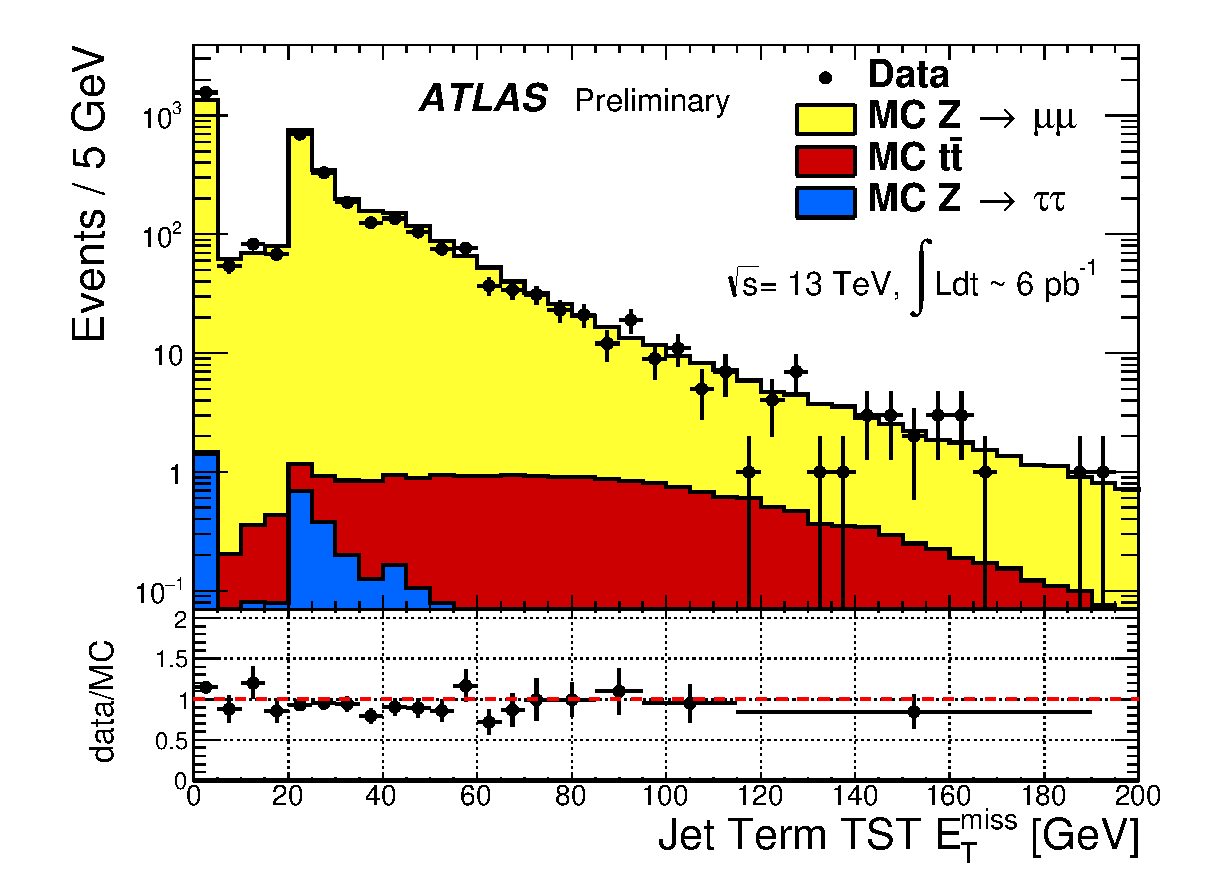
\includegraphics[width=.9\linewidth]{ATLAS-CONF-2016-078/fig_02a}}\ref{subfig:disquark_decay_tree}
\subfloat[Digluino decay tree]  {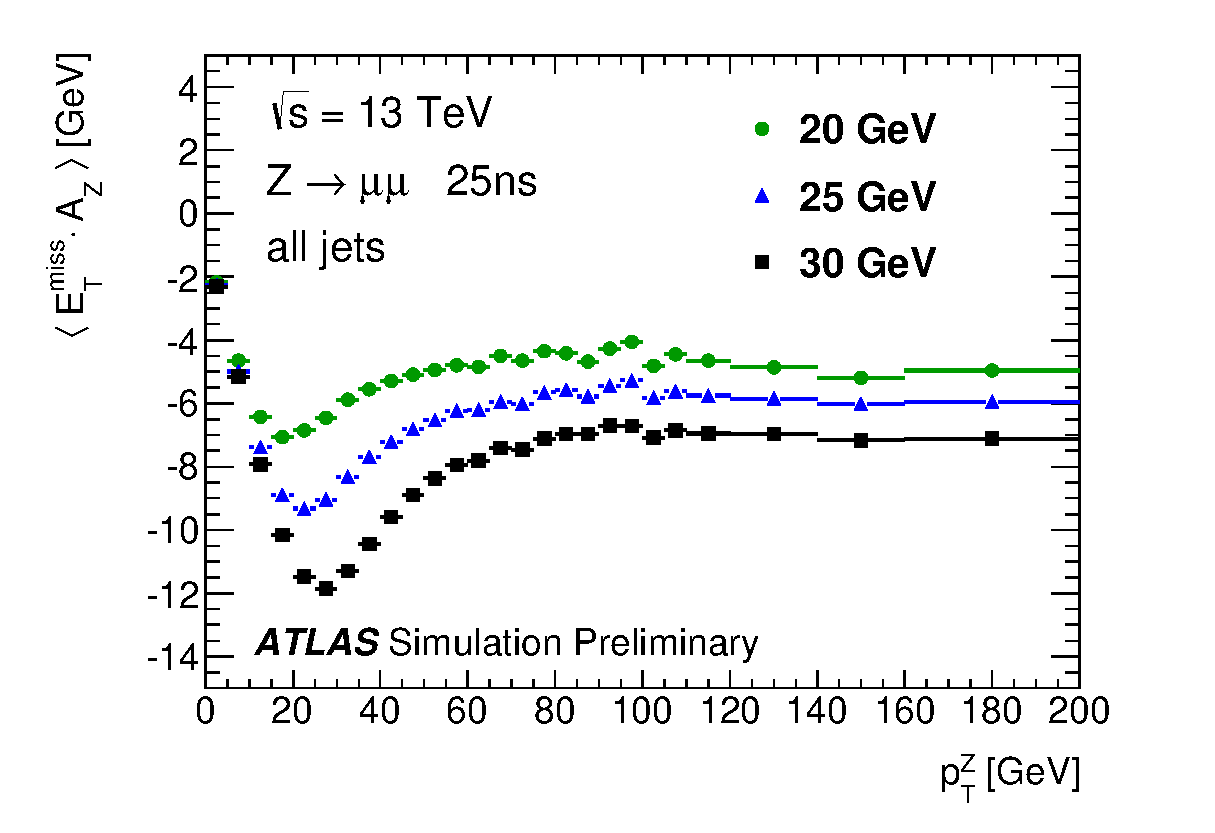
\includegraphics[width=.9\linewidth]{ATLAS-CONF-2016-078/fig_02b}}\ref{subfig:digluino_decay_tree}
\subfloat[Compressed decay tree]{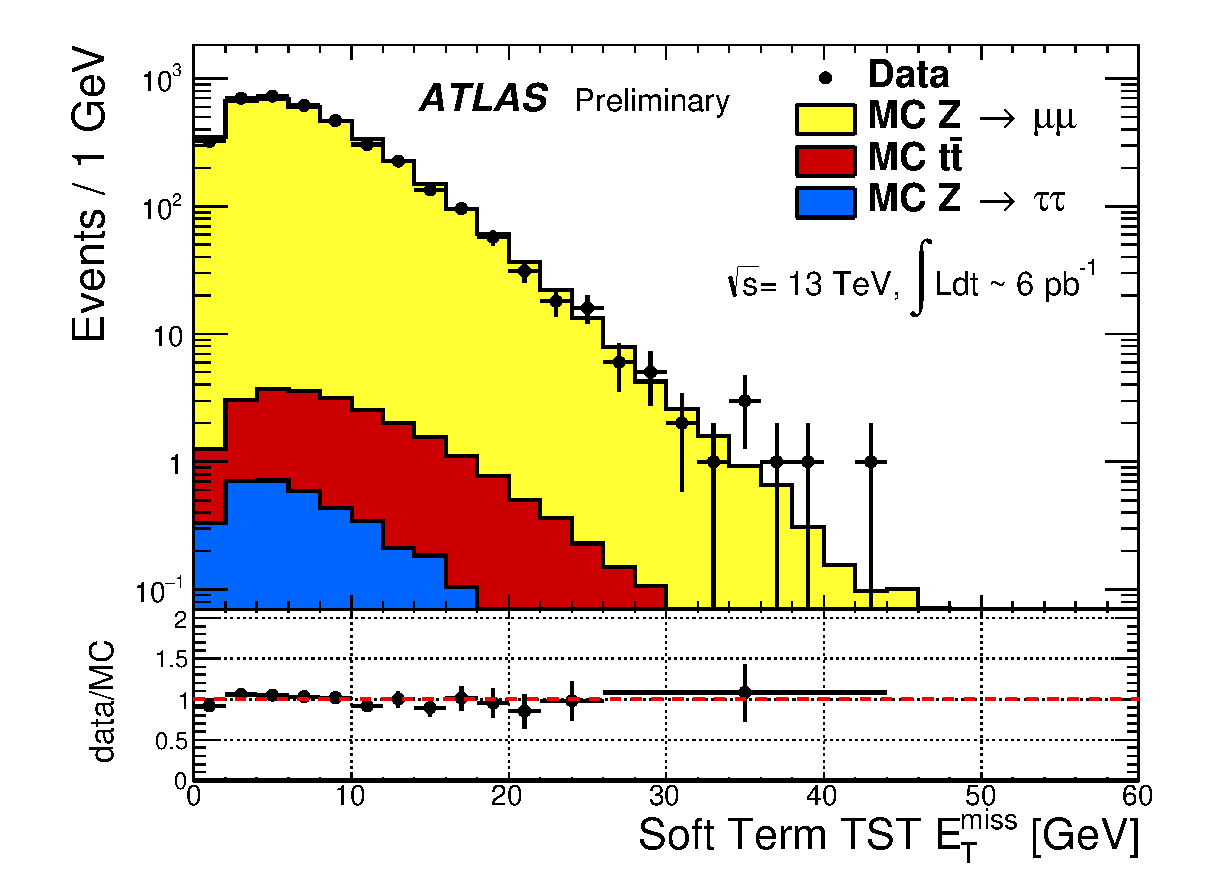
\includegraphics[width=.9\linewidth]{ATLAS-CONF-2016-078/fig_02c}}\ref{subfig:compressed_decay_tree}
\end{figure}
Leaving temporarily the question of ``how'' we apply the jigsaw rules, let us compare these trees to the signal processes of interest.
In particular, we want to compare the Feynmann diagrams of \ref{fig:feynmann_signal} with the decay trees of \ref{fig:decay_trees}.
The decay tree in \ref{subfig:disquark_decay_tree} corresponds exactly to that expected from disquark production, and matches very closely with the principles of the razor approach.
We first apply a jigsaw rule, indicated by a line, to the kinematics of the objects in the \textit{LAB} frame.
This outputs the kinematics of our event in the \textit{parent-parent} (\PP) frame, or in the razor terminology, the CM frame.
That is, the kinematics of this frame are an estimator for the kinematics in the center of mass frame of the disquark system.
We apply another jigsaw, which splits the objects in the \PP frame into two new frames, known as the \Pa and \Pb systems.
These are equivalent to the razor frames of the razor technique, and represent proxy frames where each squark is at rest.
In \Pa (\Pb), the decay is symmetric between the visible \Va (\Vb) objects and the invisible system \Ia (\Ib).
To generate the estimator of the kinematics of the \Va, \Vb, \Ia, and \Ib systems in the \Pa and \Pb systems, we apply another jigsaw rule to split the total \met between \Pa and \Pb, which allows calculations of these kinematics in these frames.
For the case of disquark production, this is the expected decay tree, and we stop the recursive calculation at that level.

In the case of digluino production, we expect two additional jets, and we can perform an additional boost in each of \Pa and \Pb, to what we call the \Ca and \Cb frames.
The decay tree is shown in \ref{subfig:digluino_decay_tree}.
In this case we apply a jigsaw at the level of \Pa (\Pb) which separates a single visible object $V_{1a}$ ($V_{2a}$) from the child frame \Ca (\Cb).
This child frame represents the hypothesized squark after the decay $\supe{g} \rightarrow g \supe{q}$, which then decays as in the squark case.
This gives additional information which will be exploited for the gluino specific search regions.

The final decay tree used in this thesis is the \textit{compressed} decay tree.
Compressed refers to signal models which have a small splitting between the mass of the proposed sparticle and the \lsp.
In this case, the sparticle decay products (i.e. the jets and \met) do not generally have large scale\cite{Jackson:2016mfb}.
Instead, the strategy is generally to look for a large-scale initial state radiation (ISR) jet which is recoiling off the disparticle system.
In the case where the LSPs receive no momentum from the sparticle decays, the following approximation holds:
\begin{align}
\met \order -p_T^{\text{ISR}} \times \frac{m_{\lsp} }{m_{\text{sparticle}}}
\end{align}
where $\pt^{\text{ISR}}$ is the transverse momentum associated to the entire ISR system.

RJR offers a natural and straightforward way to exploit this feature in events containing ISR.
One imposes the simple decay tree in \ref{subfig:compressed_decay_tree} with associated jigsaw rules.
With suitable jigsaw rules, this decay tree ``picks out'' the large \pt ISR jet, recoiling off the \met and additional radiation from the sparticle decays.
This provides a convenient set of variables to understand compressed scenarios.

In this section, we have seen how one imposes particular decay trees on an event to produce a basis of kinematic variables in the approximated frames relevant to the hypothesized sparticle decay chain.
This explains why we call this procedure ``recursive'': we can continue the procedure through as many steps of a decay tree as we want, and each application of a jigsaw rule is dependent on the variables produced in the last step.
The question, of course, is \textit{what are these jigsaw rules?}.

\subsection{Jigsaw Rules}

Jigsaw rules are the fundamental step that allow the recursive definitions of the variables of interest.
In principle, we want rules which allow us to fully define kinematic variables at each step in a decay tree.
The only possible solution to fully define the event kinematics in terms of the frames of the hypothesized decays is the imposition of external constraints to eliminate additional degrees of freedom.

In the original razor point of view, some jigsaw rules can be seen as the definitions of the boosts which relate the different frames of interest, while other rules allow one to combine multiple objects and place them into a particular hemisphere (previously megajet).
These are the two forms of jigsaw rules: combinatoric and kinematic.
As we have stressed before, the jigsaw rules are a \textit{choice}; as long as a particular jigsaw rule allows the definition of variables at each step in a decay tree, it is ``as valid'' as any other rule.

Practically speaking, in this thesis we use only a small subset of possible jigsaw rules.
The combinatoric jigsaw rule we use has already been introduced as megajet construction above.
The minimization of
\begin{align}
m_{J_1}^2 + m_{J_2}^2.
\end{align}
is a jigsaw rule to deal with the combinatoric ambiguity implicit in which jets go in which hemisphere.
This is the jigsaw rule used in the decay trees when going from one frame to two frames such as \PP $\rightarrow$ \Pa,\Pb.

We will use two other jigsaw rules, which are both kinematic jigsaw rules.
One has already been used in the razor technique.
The minimization of $\beta_L$ will be used as the jigsaw rule in the first step of each decay tree: the LAB frame to the \PP/CM frame.
This is in effect the imposition of longitudinal boost invariance, as we expect on average $p_{z,\text{\PP,CM}} = 0$.
One defines a unique longitudinal boost by imposition of this external constraint.

The final jigsaw used in this thesis was not used in the razor technique.
We describe it here.
It can be seen as the resolution of the ``amount'' of \met that ``belongs'' to each hemisphere, and therefore how to impose the transverse boost onto each of i.e. \Pa and \Pb.
Equivalently, it can be seen as the resolution of the kinematics of the \Ia and \Ib objects in the disquark and digluino decay trees.

\section{Variables used in the search for zero lepton SUSY}